\documentclass[a4paper]{report}
\usepackage{a4wide}
\usepackage{fancyhdr}
\usepackage{scrextend}
\usepackage{coordsys,logsys,color}
\usepackage[bookmarksopen,bookmarksdepth=5]{hyperref}
\usepackage{url}
\usepackage{texdraw}
\usepackage{graphicx}
\usepackage{wrapfig}
\usepackage{listings}
\usepackage{diagbox}
\usepackage{enumitem}
\usepackage{amssymb}
\usepackage{amsmath}
\usepackage{float}
\usepackage{tikz}
\usepackage{longtable}
\usepackage{booktabs}
\usepackage{ltxtable}
\usepackage{cleveref}
\usepackage[backend=biber]{biblatex}
\usepackage{minted}

\NeedsTeXFormat{LaTeX2e}
\definecolor{darkblue}{rgb}{0,0,.6}
\hypersetup{colorlinks=true, breaklinks=true, linkcolor=black, menucolor=darkblue, urlcolor=darkblue, citecolor=darkblue}

\pagestyle{fancy}
\rhead{}

\setlength{\headheight}{23pt}
\bibliography{resources.bib}

\begin{document}

\begin{titlepage}
\thispagestyle{plain}
   \begin{center}
       \vspace*{1cm}
        \Huge
        \textbf{On Dynamic Record Layout} \\ [0.5em]
        \Large
       \textbf{and a naive graph database} \\
       \vspace*{2cm}
       \normalsize
       \textbf{Fabian Klopfer \\
       Theodoros Chondrogiannis} \\ \vspace*{0.5cm}
       Database and Information Systems Group \\
       Department of Computer Science \\
       University of Konstanz\\
       
        
        \vspace*{1cm}
        
        \textbf{Abstract}
        
   \end{center}
\end{titlepage}

\newpage
\tableofcontents


\chapter{User Guide}
\section{Introduction}
\begin{center}
    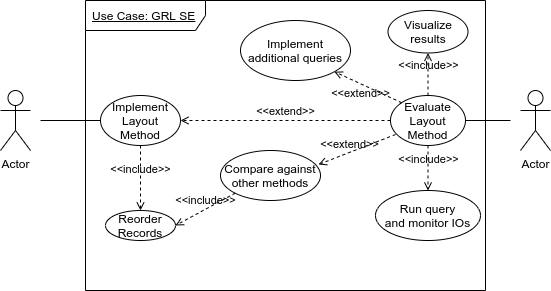
\includegraphics[keepaspectratio,width=.7\textwidth]{img/use_case.png}
\end{center}
		
\begin{center}
 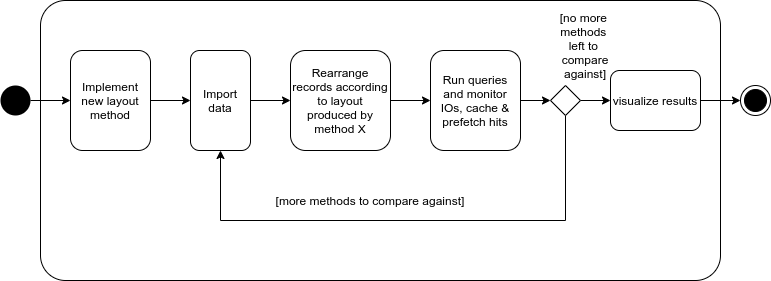
\includegraphics[keepaspectratio, width=1\textwidth, height=\textheight]{img/activity.png}
\end{center} 

\section{Graph Database}

\subsection{Architectural Overview}
\hspace{-2cm}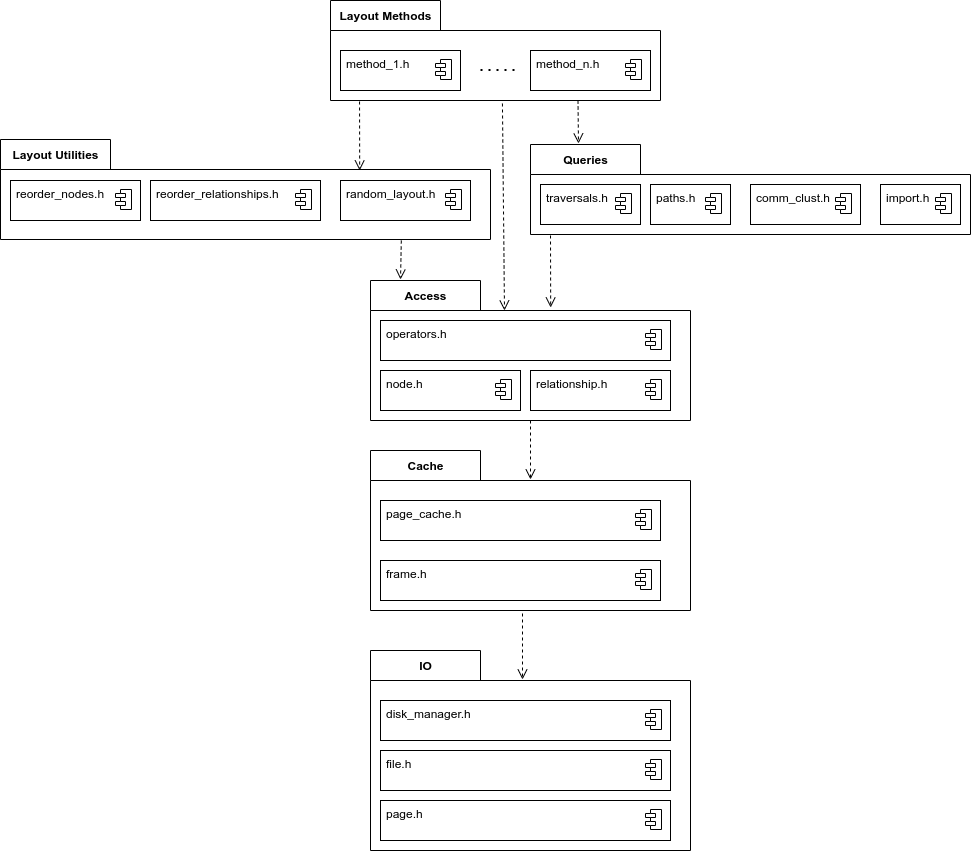
\includegraphics[keepaspectratio,width=1.2\textwidth, height=.7\textheight]{img/overview.png}



\subsection{Building}

\subsection{Tests \& Coverage}



 
\section{Record Layout Methods}

\subsection{Theoretical Aspects}

\subsection{Static Layout}

\subsection{Dynamic Layout}

 \subsection{Benchmarks}
    \subsubsection{Traversal-based Queries}
    The currently implemented benchmark provides a stepwise less branching traversal of the graph. While BFS and DFS are the most branching traversal possible and Dijkstra resembles this, it depends on the heuristic of A$^*$ how branching it is. With the zero heuristic it resembles Dijkstra's, with the perfect heuristic (actual distance to target vertex from source vertex) it does not branch at all (only the neccessary nodes are visited). ALT provides a good heuristic but not a perfect one. \\
    To conclude: The benchmark tests how well the particular record layout deals with the branching factor od the traversal. \\
    A neighbourhood-based layout should perform well for BFS-based traversals but could possibly degrade for a non-branching or DFS traversal. \\
    An access history-based layout should work well for repeated queries of the same path for example.
    
    
 \subsection{Visualizations}
    \paragraph{Total Accesses per Query per Method}
    A bar diagram that shows the number of disk accesses for a set of queries and possibly many methods. Reasonable if you want to compare the performance of different layouts on the same set of queries.
    
    \paragraph{Access sequence} Visualizes the addresses that are accessed as a line chart to inversigate if the access is sequential or ``jumps'' a lot. Samples 50 consecutive accesses at random.



\section{Conclusion}


\printbibliography

\addtocontents{toc}{\protect\setcounter{tocdepth}{2}}

\chapter{Software Requirement Specification and Design Document}
\begin{refsection}
\section{Introduction}
	\subsection{Purpose}
			The purpose of this combined Software Requirements Specification and Design Documents is to describe the features, constraints, demands and the intended design of a research environment for the optimal layout of graph records on disk in detail. This document is intended for both the stakeholders and the developers of the system and will be proposed to Dr. Theodoros Chondrogiannis, the supervising postdoctoral researcher.
	\subsection{Scope}
			This Software system shall implement a graph record layout research environment, that consists of a graph database along with tools, that rearranges the recrods of the database based on a predefined format, measure the number of disk accesses needed to service a certain query and that provide other layouts to compare against. The time frame is three months, distributed over four months with $75\%$ work load. When the system is implemented, a specific method that is to be dervied shall be too implemented, evaluated and published within the same time frame.

    \subsubsection{Definitions, Acronyms, Abbreviations}
	\begin{longtable}{|>{\raggedright \arraybackslash}p{0.35\textwidth}||
	>{\raggedright \arraybackslash}p{0.15\textwidth}|>{\raggedright \arraybackslash}p{0.5\textwidth}|} \hline

	word & shortform & meaning \\ \hline
	database & db & a software system to store and alter data in an organized manner. \\ \hline
	Operating System & os & An operating system is system software that manages computer hardware, software resources, and provides common services for computer programs. \\ \hline
    Portable Operating System Interface & POSIX & A specification for a set of OSes that covers for example Linux, macOS and BSD-style operating systems. \\ \hline
	C Programming Language & C & a programming language. \\ \hline
	Input/Output & IO & the notion of loading and storing information to media other than RAM and CPU registers. In this document hard drive and solid state disk are meant primarily. \\ \hline
	Create, read, update, delete & CRUD & The basic database operations, that allow to create, read, update and delete a record. \\ \hline
	Databases and Information Systems & DBIS & The name of the group at the university of Konstanz, at which the software system is build. \\ \hline
	Stanford Network Analytics Project & SNAP & A porject of the university of stanford that hosts many large scale graph data sets.  \\ \hline
	Least Recently Used & LRU & A strategy when evicting pages from a pool of memory. \\ \hline
	Breadth-first Search & BFS & A graph traversal scheme, where all neighbours of the current node are visited before continuing with the next node. \\ \hline
	Depth-first Search & DFS & A graph traversal scheme, where the next node is considered before visiting all neighbours of the current node. \\ \hline
	Single Source Shortest Path & SSSP & The problem of finding the shortest path to all nodes in a graph from one source node. \\ \hline
	\end{longtable}

	\subsubsection{Overview}
		In the second section several conditions, assumptions and circumstances will be mentioned, that help charachterizing the software's special use case. In the thrid chapter the concrete requirements are listed. The fith section outlines an overview of the proposed software architecture. The sixth section, finally, elaborates on the subsystems of the archtiecture.

		
\subsection{Overall description}
	\subsubsection{Product Perspective}
		The product shall rely on functions of unixoid OSes. 
		That is it uses the interfaces specified by the OpenGroup in the POSIX.1-2017 specification (also called IEEE Std 1003.1-2017)~\autocite{posix}.
		There are no relations to other software systems than the operating system during the runtime of the environment.

	\subsubsection{Product Functions}
	The product shall support different tasks in graph record layout research: 
		\begin{enumerate}
		 \item Import data into a graph database.
		 \item Query the database with a certain fixed function.
		 \item Rearange the record layout on disk with a layout given in a specific format.
		 \item Monitor the number of disk IOs.
		 \item Monitor the caching behaviour.
		 \item Provide interfaces for the implementation of new layout methods.
		 \item Provide a interfaces to ease the implementation of new queries.
		\end{enumerate}
		
        This shall be done using a graph database, that shall save related information to disk and load them into a cache on access, as well as support the common CRUD functionality. \\
        

	\subsubsection{User Characteristics}
		The potential users are the staff and student assistants of the DBIS group. Therefore standard user will have technical knowldege, and have visited at least a basic course on databases. Futher the users are able to program in C.
		There are three different types of users of this research environment: \\
		\begin{itemize}
			\item Researchers: Implements new layout method, benchmarks the result of the method against other layouts, visualizes the result of the benchmark. Should at least know the theory of how records are stored.
			
		 	\item Supervisors: Works on the administration and coordination of the project. Eventually hires other researchers and developers. Also a researcher.
		 	\item (Future) Developers: Uses the existing framework to extend the functionality, for example to implement additional queries of a different type, add new features like storing properties and similar things. Needs to know details of database architecture and implementation, more advanced C programming and some software engineering.
		\end{itemize}
		\begin{center}
		 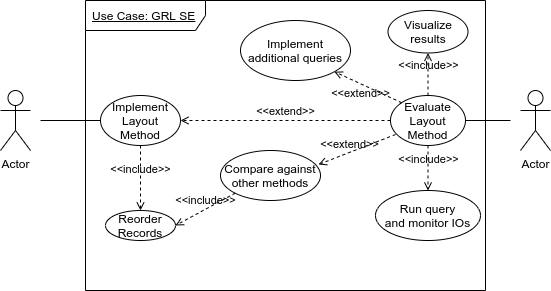
\includegraphics[keepaspectratio,width=0.8\textwidth]{img/use_case.png}
		\end{center}

	\subsubsection{Constraints}
		\begin{itemize}
			\item The database is expected to be run on a standard notebook and desktop machine, that is it needs to run without momory-related errors on a machine with 8 GiB RAM, no matter the data set size.
		\end{itemize}

	\subsubsection{Assumptions, Dependencies \& References}
		The environment supports only POSIX-compliant OSes. \\
		A documentation of the low-level design of Neo4J based on Michael Brendle's work and the source code of Neo4J at revision 4.1~\autocite{GitHubneo4j} is referenced and can be found in the folder \mintinline{bash}{doc/neo4jstorage}.



\section{Requirement Specification}
	\subsection{External interfaces}
	The POSIX interfaces. \\
	The data format of some of the SNAP data sets. \\

	\subsection{Functional requirements}
\begin{enumerate}[label*=\arabic*]
\item Data Storage and IO \\
    The system shall
	\begin{enumerate}[label*=\arabic*]
	\item store a graph $G$ consisting of nodes and edges $(V, E)$.
	\item store the records in a file on disk.
    \item be able to grow and shrink the size of the file that is used.
    \item be able to read from disk.
    \item be able to write information to disk.
	\end{enumerate}
	
\item Data Caching and Memory  \\
    The system shall
	\begin{enumerate}[label*=\arabic*]
	\item not exceed a certain memory limit for both pages from disk and memory requirements from queries.
	\item split an amount of memory into frames.
	\item load data from disk into a frame on request.
	\item maintain information on unused frames.
	\item maintain a mapping from loaded data to frames.
	\item evict data from memory when the memory limit is hit
	\item be able to prefetch by reading more data than required in a neighbourhood
    \item be able to monitor the numer of overall disk accesses.
	\item be able to monitor the number of disk accesses that are necessary, if only a certain limited amount of memory is available.
	\item be able to monitor the cache hit rate.
	\item be able to monitor the prefetch hit rate.
	\end{enumerate}

\item Data Access \\
    The system shall
	\begin{enumerate}[label*=\arabic*]
    \item be able to calculate the location in the file of nodes and relationships efficiently
    \item keep track of free record slots on disk.
	\item be able to create, read, update and write nodes.
	\item be able to create, read, update and write relationships.
	\item provide an interface to easily retrieve and traverse data.
    \item provide functions to retrieve common informations about nodes and relationships, like the node degree.
	\end{enumerate}

\item Queries \\
    The system shall
	\begin{enumerate}[label*=\arabic*]
	\item implement the most basic traversal schemes --- BFS and DFS.
	\item implement Dijksta's algorithm for finding all shortest paths from a single source (SSSP).
	\item implement the A$^*$ algorithm for the shortest path problem.
	\item implement the ALT algorithm for the shortest path problem.
	\item provide data structures for the results of the above algorithms.
	\item implement the Louvain method for community detection.
	\item implement a random walk.
	\item be able to import a set of standard data sets from the SNAP data set collection.
	\end{enumerate}

\item Layout Tools \\
    The system shall
\begin{enumerate}[label*=\arabic*]
	\item provide a function to generate a randomized record layout.
	\item provide functions to reorganize the record layout on disk, given updated record IDs.
	\item provide a function to reorganize the relationships given a layout of the vertices.
	\item provide a function to sort the incidence list structure after reorganizing the record structure.
\end{enumerate}

\item Layout Methods \\
    The system shall
\begin{enumerate}[label*=\arabic*]
	\item implement one static and one dynamic history-based layout method for a static database.
	\item provide an interface for implementing new layout methods.
\end{enumerate}
\end{enumerate}

\subsection{Performance Requirements}
\begin{enumerate}[label*=\arabic*]
		\item The system shall work with limited RAM resources even for very large datasets.
\end{enumerate}

\subsection{Software System Attributes}
\begin{enumerate}[label*=\arabic*]
    \item Maintainability
    \item Extensibility
    \item Correctness
\end{enumerate} \vspace{2em}
		
		
\begin{center}
 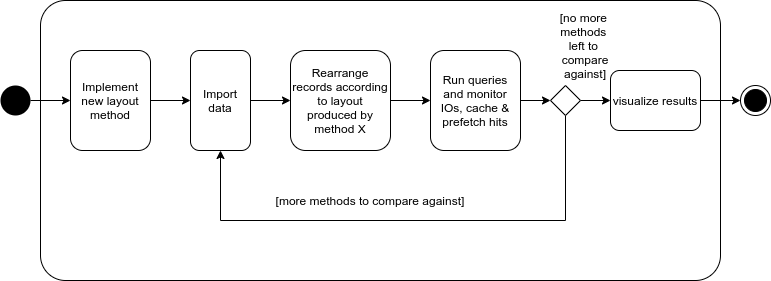
\includegraphics[keepaspectratio, width=1\textwidth, height=\textheight]{img/activity.png}
\end{center}
		\newpage
		
\section{Software Design}
\subsection{Overview}
The graph record layout research environment consists of the lower layers of a database and a set of functions to assist in reordering records, measuring the number of IOs of a certain layout, visualizing the results, queries with certain access patterns, and an interface to implement new layout methods easily into the environment. The database layers are implemented in the IO, Cache and Access layers. The Query package does not contain a complete query language and evaluator but just a set of algorithms to be executed on the graph. \\ [2em]

\hspace{-2cm}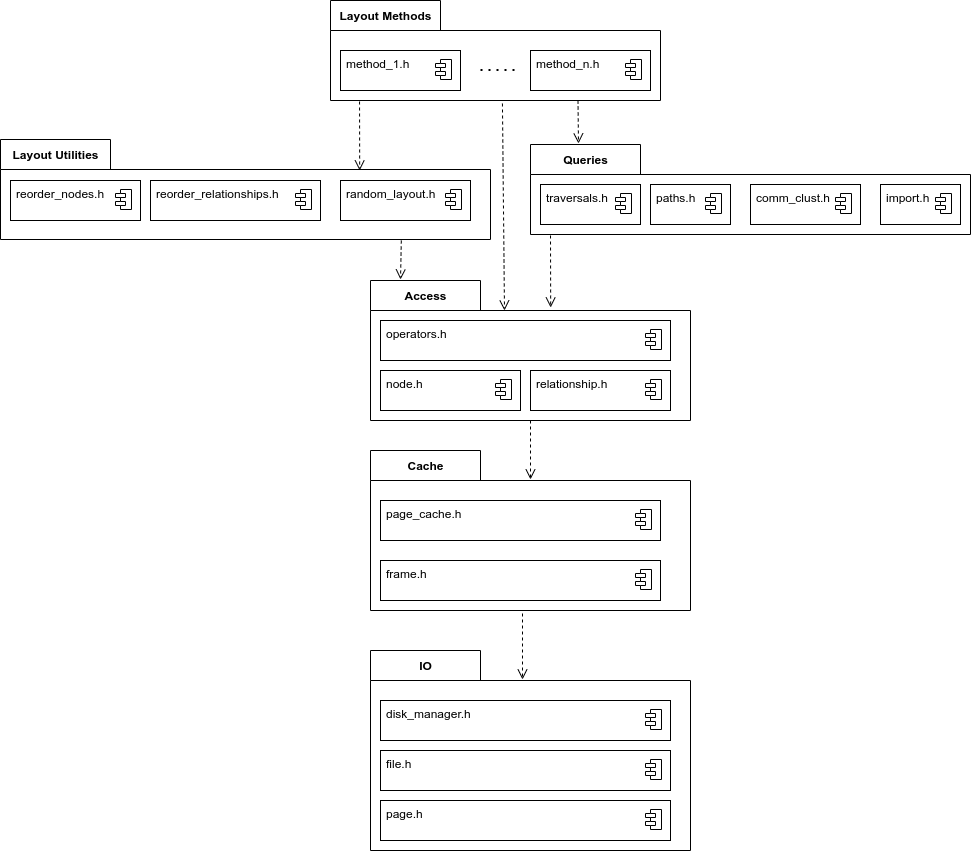
\includegraphics[keepaspectratio,width=1.2\textwidth, height=.7\textheight]{img/overview.png}

\newpage

\subsection{Subsystem decomposition}
    \subsubsection{IO}
        The IO package shall provide the concepts of a disk file and the disk manager. \\
        Each file consists of a set of pages. The file accounts for the usage of pages with a page directory~\autocite{ramakrishnan2000database}. It also provides functions to read and write a page. \\
        The database stores its data in the slots contained in the pages contained in the files. The files are created, grown and shrinked by the disk space manager.   \\
        
        \begin{center}
         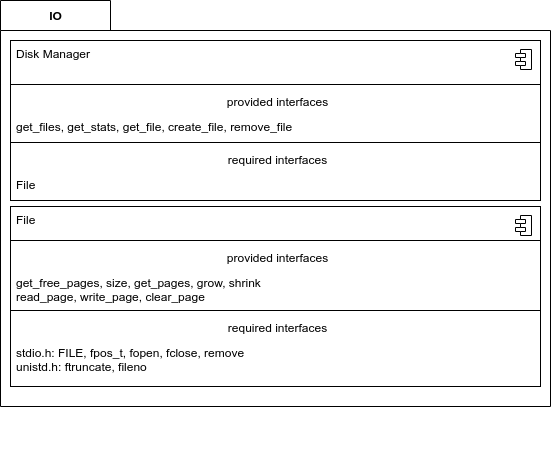
\includegraphics[keepaspectratio, width=\textwidth, height=0.3\textheight]{img/io_arch.png} \\
        \end{center}

    \subsubsection{Page Cache}
        This packages provides a cache for pages, that is it loads and stores pages from or to disk in a fixed amount of RAM. To do this it splits the available main memory into frames of the size of a page and maintains a mapping from frames to pages, a list of free frames and evicts pages from main memory to free up space for pages to be loaded. Each page consists of slots that can hold records. The page keeps track of the usage of these slots with a bitmap. \\
        \begin{center}
         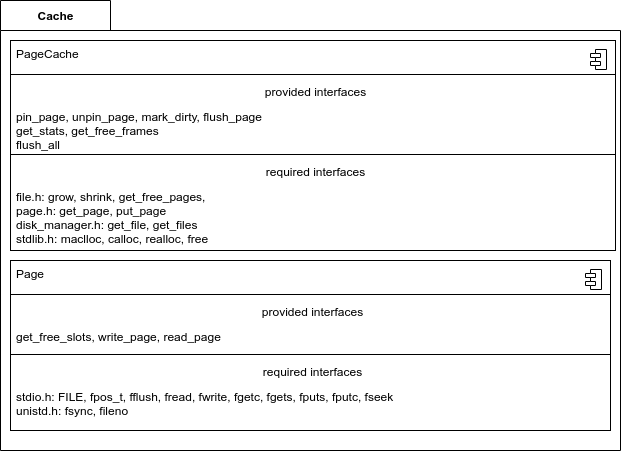
\includegraphics[keepaspectratio, width=\textwidth, height=0.3\textheight]{img/cache_arch.png} \\
        \end{center}
        \newpage
        
    \subsubsection{Access}
        The Accesss package provides the record structures along with methods to create, read, update and delete nodes and relationships. The records structs are inspired by the ones used in Neo4 (see the documentation on that).  It futher provides these functions for all records and ranges of records at once. Finally it implements the expand operator as described by Grossniklaus and Hoelsch~\autocite{Holsch2016Algeb}.

        \begin{center}
         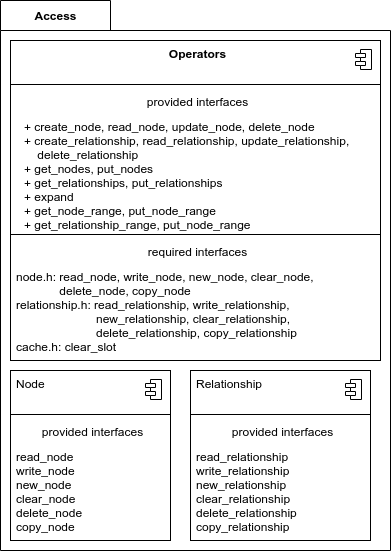
\includegraphics[keepaspectratio, width=\textwidth, height=0.5\textheight]{img/access_arch.png} \\
        \end{center}

            
    \subsubsection{Queries}
        The query package is a collection of algorithms to be executed using the lower levels of the graph database. These include traversals, shortest path algorithms, community detection methods, but also a utility to import datasets from the stanford network analytics platform project~\autocite{snap}. \\
        Currently implemented are:
        \begin{itemize}
         \item Traversals
         \begin{itemize}
                \item BFS~\autocite{zuse1948allgemeinen}
                \item DFS~\autocite{lucas1891recreations}
                \item Random Walk~\autocite{pearson1905problem}
               \end{itemize}
         \item Shortest Path
         \begin{itemize}
          \item Dijksta's Algorithm~\autocite{dijkstra1959note}
          \item A$^*$~\autocite{hart1968formal}
          \item ALT~\autocite{goldberg2005computing}
         \end{itemize}
        \item Community Detection
        \begin{itemize}
         \item Louvain Method~\autocite{blondel2008fast}
        \end{itemize}

        \end{itemize}

        
    \subsubsection{Layout Utilities}
    The layout utilities package provides functions to reorder the records given a mapping from the current record IDs to the desired ones. It also provides means to generate a random mapping and to sort the incidence list of the relationships after reorganizing the records.
    
    \subsubsection{Layout Method Interface} 
    The layout method interface is to be implemented, such that it returns a map from the current IDs to the desired record IDs, where the record IDs encode the position in the file. The name of the method can be arbitrary, it is just of importance that the arguments and the return type are as specified, as well as the invariants.
    \begin{verbatim}
  unsigned long[] layout_nodes(graph_database db) {
    require db != null;
    require db.num_nodes > 0;
    ensure db.num_nodes == result array length
    ensure unique node IDs
  }
  
   unsigned long[] layout_relationships(graph_database db) {
    require db != null;
    require db.num_nodes > 0;
    require db.num_relationships > 0;
    ensure db.num_relationships == result array length
    ensure unique relationship IDs
  }
\end{verbatim}

\subsubsection{Visualization Utilities}
Finally a python script provides means of visualizing the number of IOs and the cache hit rate as monitored by the page cache package. It relies on matplotlib and numpy.

\printbibliography
\end{refsection}
\end{document}
